\section{Architectures}
In questa prima sezione verranno esaminate le varie architetture che sono state progettate e sintetizzate per il moltiplicatore floating point

\subsection{Classic Architecture}
Il punto di partenza della progettazione è stato il floating point pipelined multiplier a 32 bit, del quale è stato fornito il codice vhdl.
Lo schema di massima è mostrato in \autoref{fig:mult_struct}, è suddiviso in 4 stage principali:
\begin{itemize}
\item Stage 1: Viene effettuato l'unpacking dei due numeri floating point in ingresso.
\item Stage 2: Viene effettuata la moltiplicazione dei significands, trattati come numeri interi.
\item Stage 3: Viene effettuato il rounding dei significands.
\item Stage 4: Viene effettuato il calcolo dell'esponente e infine viene trasformato nuovamente il numero in floating point tramite il blocco di packing.
\end{itemize}

\begin{figure}[h]
	\center
	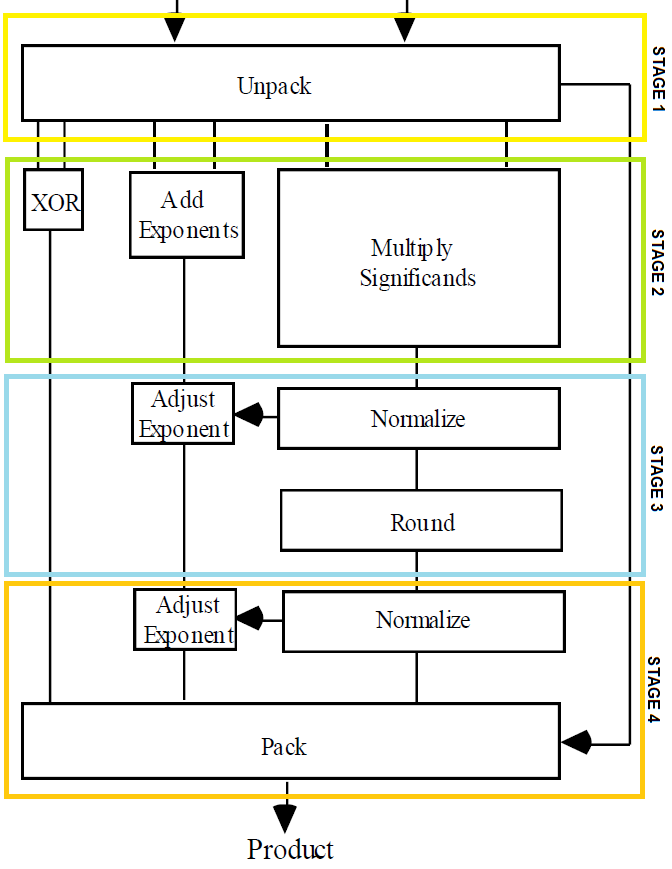
\includegraphics[width=0.6\textwidth]{mult_structure.png}
	\caption{Structure of the floating point multiplier}
	\label{fig:mult_struct}
\end{figure}

\noindent Studiando il codice VHDL si nota inolte che tra uno stadio e l'altro sono sempre presenti dei registri che campionano il segnale sul fronte di salita del clock. Per questo si può affermare che gli stage funzionali corrispondono agli stage di pipeline.
\todo{E'GIUSTO?}
Un'altra osservazione che è possibile fare su questa architettura standard è che nel secondo stage, il tipo di moltiplicatore utilizzato per moltiplicare i significands non è specificato infatti è presente un process nel quale viene fatta l'operazione con il simbolo "*" che lascia completa libertà al sintetizzatore nella scelta dell'implementazione hardware.

\subsubsection{Testbench}

Prima di partire con le varie modifiche dell'hardware è stato simulato tramite Modelsim il corretto funzionamento del circuito fornito. E' stato creato un testbench in verilog con i blocchi relativi alla generazione degli input, al DUT e al salvataggio degli output.
Come file di ingresso è stato utilizzato quello fornito sia per l'ingresso $A$ sia per $B$ di conseguenza il moltiplicatore effettuava il quadrato del numero in questione. I numeri erano rappresentati su 8 bit esadecimali quindi prima di fornirli al DUT è stata effettuata la conversione in binario.
Infine, confrontando i risultati ottenuti con quelli forniti come esempio, è stato possibile confermare il funzionamento del circuito. Inoltre studiando il timing generato da Modelsim si nota come effettivamente la latenza del circuito sia quella ipotizzata.
\\
\todo{GIUSTO?}
Successivamente è stato modificato il codice VHDL in modo da aggiungere ai segnali di ingresso dei registri; questa correzione serve a svincolare il timing degli ingressi, con eventuali glitch, dal timing interno del circuito.
A fronte di questa modifica è stato effettuato un secondo testbench, funzionalmente uguale al precedente, che ha mostrato anche in questo caso che il circuito sotto esame funzionasse correttamente.

%%%%%%%%%%%%%%STAGE 2 MANIPULATION%%%%%%%%%%%%%%%

\subsection{Stage 2 CSA PPARCH}
In this section a few optimizations was done. In fact, respect to the classic architecture there are several differences that change the circuit behavior. The CSA architecture is implemented by using the \textit{Carry Save Adders} and in the PPARCH architecture there is a \textit{pipelined} version of the stage 2. These variations can be carried out by simply using different commands during the compilation process. The stage 2 was forced to be syntetized as CSA and to do that the following commands were used in the synthesis process:
\begin{itemize}
\item ungroup -all flatten
\item set\_implementation DW02\_mult/csa [find cell *mult] 
\end{itemize}
For the PPARCH the same commands were used, but with a difference in the mult options:
\begin{itemize}
\item ungroup -all flatten
\item set\_implementation DW02\_mult/pparch [find cell *mult] 
\end{itemize}
The area and the minimum period estimation was the goals of the synthesis process. The results obtained from the commands \textit{report\_area} e \textit{report\_timing} are showed in \autoref{tab:syn_results}. The \textit{CSA} architecture is roughly three times slower and the area is much greater than the \textit{PPARCH} one. Although the higher latency, the \textit{PPARCH} is a better architecture respect to the \textit{CSA} one.
Both architectures were tested in order to check the correct behavior. A testbench was used to do that and the following table shows what the output gave:

\begin{table}[H]
\begin{center}
\begin{tabular}{|c|c|c|c|}				\hline
CSA		 	  & PPARCH 					\\ \hline
00000000   	  & 00000000               	\\ \hline
3DC3910D      & 00000000                \\ \hline
0BC80005      & 00000000                \\ \hline
3F278DDF      & 00000000                \\ \hline
0B100005      & 00000000                  \\ \hline
3F800000      & 00000000                  \\ \hline
0C440004      & 00000000                   \\ \hline
3F278DDF      & 3DC3910D                  \\ \hline
0DA20000      & 0BC80005                   \\ \hline
3DC3910D      & 3F278DDF                  \\ \hline
3DC3910D      & 3F800000                   \\ \hline
3DC3910D      & 0C440004                   \\ \hline
3DC3910D      & 3F278DDF                   \\ \hline
3DC3910D      & 0DA20000                   \\ \hline
3DC3910D      & 3DC3910D                   \\ \hline
3DC3910D      & 3DC3910D                   \\ \hline
\end{tabular}
\end{center}
\end{table}

The \textit{PPARCH} architecture has a greater latency due to the pipe stages and as the table illustrates six more sets of zeros than the CSA architecture are present in output. Once the input stream reaches the end of file, the output remains the same as long as the simulation runs, in fact the output remains equal to the string \textit{3DC3910D}. In conclusion both the architectures work, but they work in a different way due to the internal structure.

%%%%%%%%%FINE-GRAIN PIPELINING%%%%%%%%%%%%%

\subsection{Fine grain pipelining}
The next aim is to modify the VHDL file by inserting a \textit{pipeline stage} in output of the stage 2, as the following image shows:
\begin{figure}[H]
	\center
	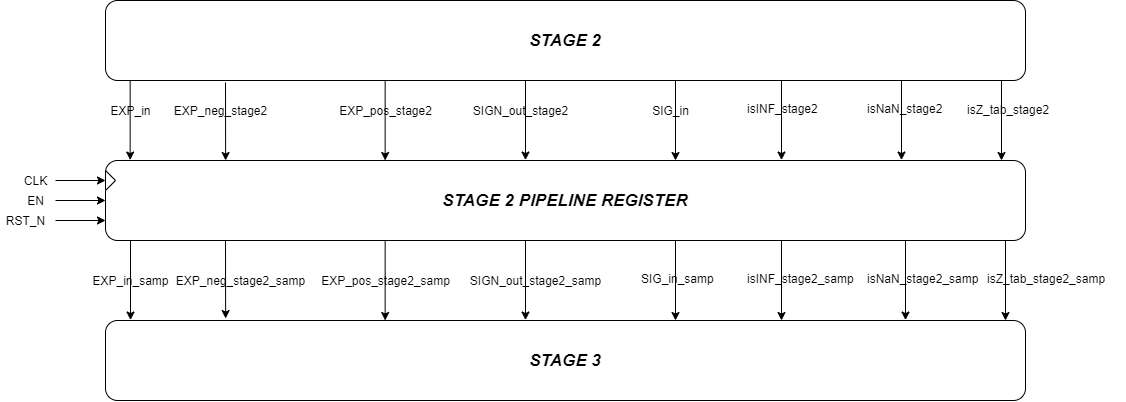
\includegraphics[width=0.9\textwidth]{Fine grain pipelining.png}
	\caption{Fine grain pipelining block diagram}
	\label{fig:mult_struct}
\end{figure}
The output register has been implemented in the VHDL file by using several registers and \textit{flip-flops} in order to ensure the correct behavior and timing.  After the VHDL manipulation, two different synthesis processes were made by using two different commands per time. In the first run, the compile command was launched after \textit{optimize\_registers} command. In the second run  \textit{compile\_ultra} was used rather than \textit{optimize\_registers} and \textit{compile}. The Synthetizer elaborates the structures in a different way, by using some algorithms instead other ones. The results in terms of timing and area are showed in \autoref{tab:syn_results}.The \textit{compile\_ultra} gave a lower area but the circuit is clearly slower respect to the one obtained by using \textit{optimize\_registers}.
\subsection{MBE}
\todo{spigare struttura MBE , Dadda}
\subsubsection{Testbench}
